<<<<<<< HEAD
Looking at the emails dataset, there are 1906 of people who received emails from Hillary. We selected the 10 receivers who received the highest numbers of emails from Clinton directly.
A simple word cloud for the emails received by these 10 accounts can be seen below:

\begin{figure}[h!]
    \centering
    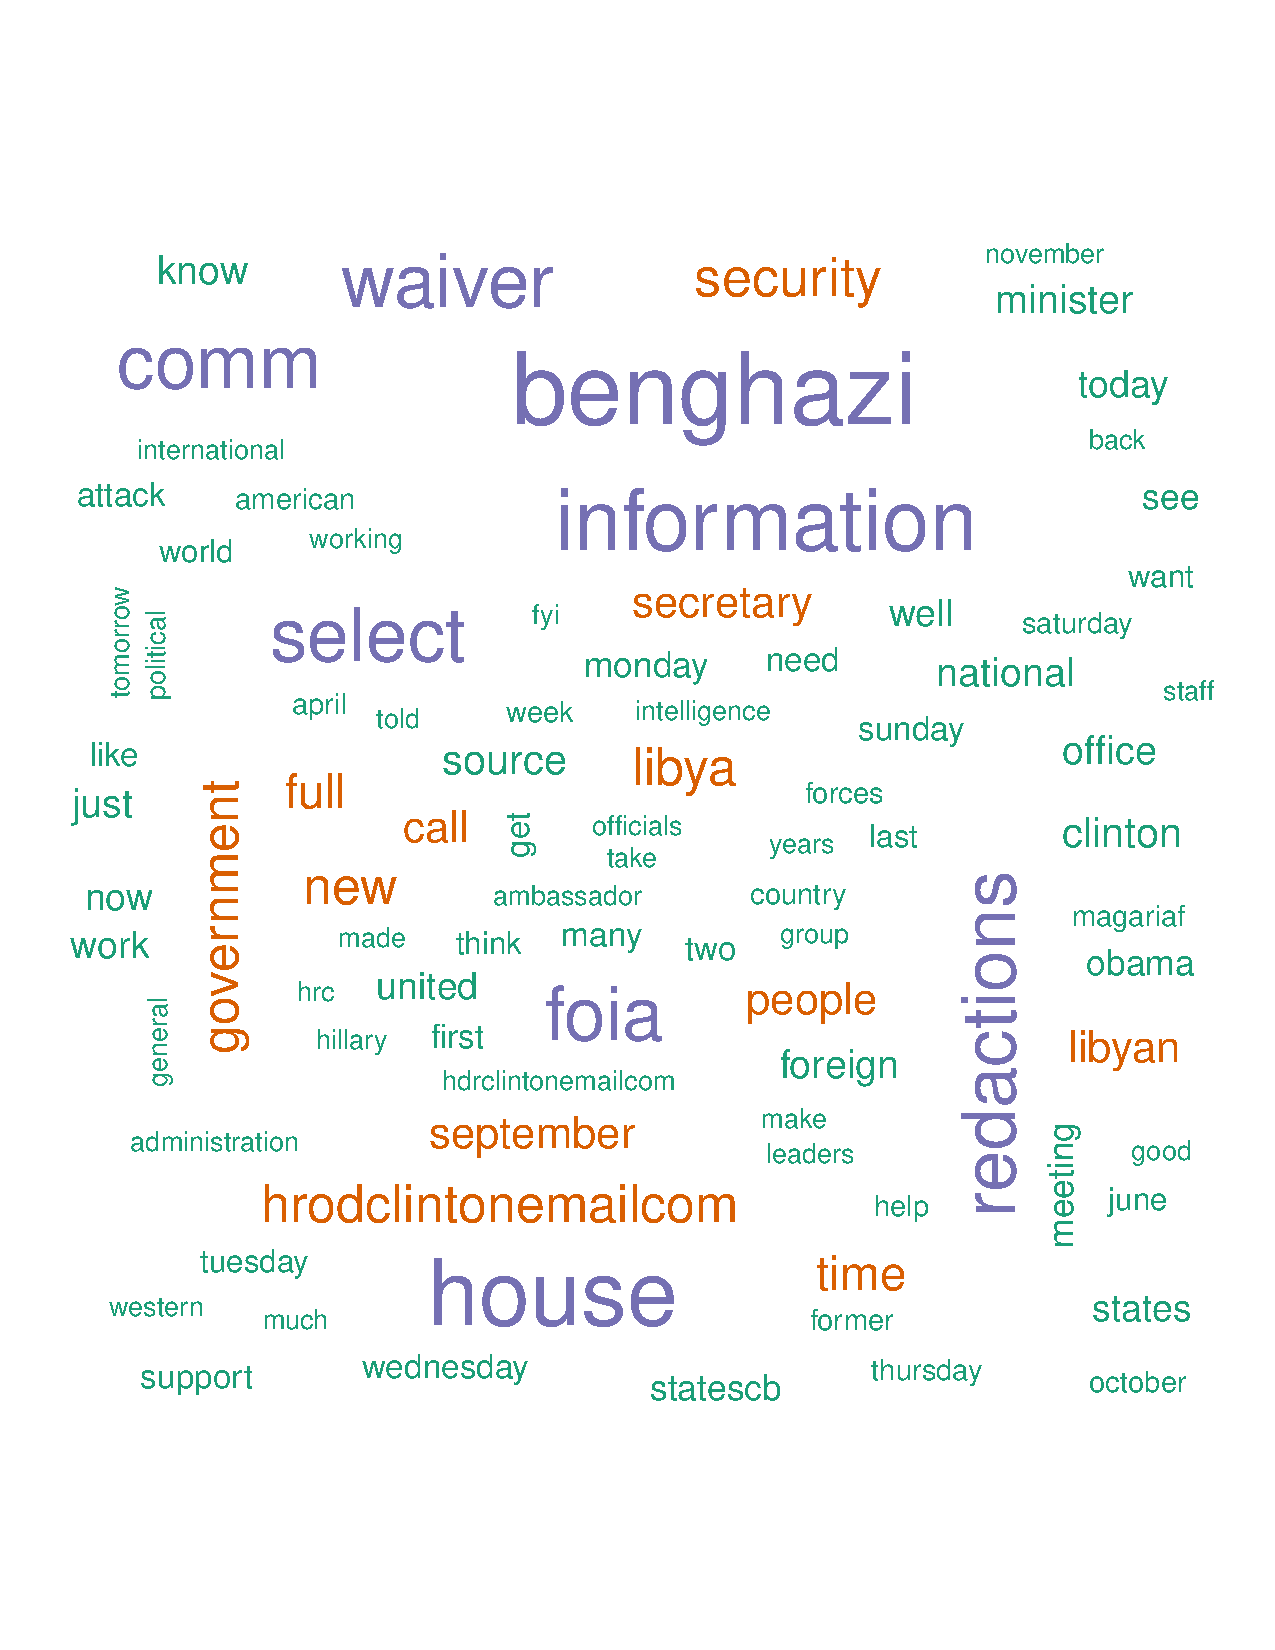
\includegraphics[width=10cm,height=10cm]
    {daitong_and_yihe/wcloud.pdf}
    \caption{Word Cloud of Emails}
\end{figure}

These receivers are a mix of both work email addresses and personal addresses. For example, Huma Mahmood Abedin, the vice chair of Hillary Clinton's 2016 presidential campaign, received 331 emails through her work email address abedinh@state.gov and 31 through her personal email. 
The list of the top 10 email receivers is shown below:
\begin{center}
  \begin{tabular}{ |l| l | c | c |c|}
    \hline
    &Name & Email Type & Frequency & Word count (cleaned)\\ \hline
    1&Huma Mahmood Abedin & Work & 331 & 981 \\ \hline
    2&Cheryl D. Mills & Work & 297 &16145 \\ \hline
    3&Jacob Jeremiah Sullivan & Work & 288 & 1696\\ \hline
    4&Lauren Jiloty & Work & 223 &1993\\ \hline
    5&Lona Valmoro & Work & 129 &8584\\ \hline
    6&Philippe I. Reines & Personal & 49 &15114\\ \hline
    7&Sidney Stone Blumenthal & Personal & 47 &2068\\ \hline
    8&Cheryl D. Mills & Personal & 35 &1786\\ \hline
    9&Monica R. Hanley & Work & 33 &13190\\ \hline
    10&Huma Mahmood Abedin & Personal & 31&6279 \\
    \hline
  \end{tabular}
\end{center}
\\\\
The typical length of emails varies wildly independent of the number of emails each account received. We can see some patterns from the table above based on the word count. Clinton sent out more lengthy emails to Sidney Blumenthal (personal), Cheryl Mills (personal) and Monica Hanley (work). It makes sense by considering the nature of their connections to HC. 
According to Wikipedia, Blumenthal is a journalist specializing in foreign policy, a former aide to President Bill Clinton, and a long-time confidant to Hillary. Mills is a lawyer who previously defended Bill Clinton in the 1999 impeachment trial and Hanley is Hillary's assistant at the state department.

The table below summarizes the roles or occupations of these 8 key persons in relation to Hillary:
\\\\
\begin{center}
 \begin{tabular}{ |l|l| } 
  \hline
   Roles & Names  \\
   \hline
\multirow{Special Assistant} 
& Lauren Jiloty \\ & Lona Valmoro \\ & Monica Hanley  \\ 
\hline
\multirow{Senior Policy Advisor} 
& Philippe Reines \\& Jacob Sullivan \\ 
\hline
\multirow{Political Journalist} 
& Sidney Blumenthal \\ 
\hline
\multirow{Lawyer} & Cheryl Mills \\
\hline
\multirow{Political Staffer} & Huma Abedin \\ 
\hline
\end{tabular}
\end{center}

Huma Abedin received the highest amount of emails from Hillary, though these were mainly brief. She served as the Vice Chair for Hillary's 2016 presidential campaign and was previously the Deputy Chief of Staff to Secretary of State Hillary Clinton from 2009 to 2013. The two senior advisors also have deep connections to Hillary. Jacob Sullivan specializes in foreign policy and was an advisor to Hillary during the campaign. Philippe Reines served as the Deputy Assistant Secretary of State for Strategic Communications in 2010 and was a senior advisor to Secretary of State Hillary Clinton in 2009. Other accounts that have received frequent emails from Clinton are Anne-Marie Slaughter, Richard Verma, Robert Russo, and Lissa Muscatine (speech writer), all of whom received under 30 emails each. 

Although the word counts already reflect Hillary's language style to different people in some sense, we would like to carry out the cluster analysis in terms of text similarities to answer questions like: 
\begin{enumerate}
  \item Does Hillary talk about similar key issues to certain (group of) people?
  \item Can we separate emails sent to private accounts from the emails sent to work accounts based only on the language used?
\end{enumerate}

After obtaining the matrix containing the distances between each pair of document, we tried two clustering methods: hierarchical clustering and K-means. 

For hierarchical clustering, we used ward.D or the Ward's minimum variance method. Figure 2 is a cluster dendrogram of the top 10 email accounts. The different colors represent the grouping. The height represents the distance between each document. For example, at the distance of 800 we can separate the group into pink and non-pink subgroups. The calculation of distance is explained in the section above.
\begin{figure}[h!]
    \centering
    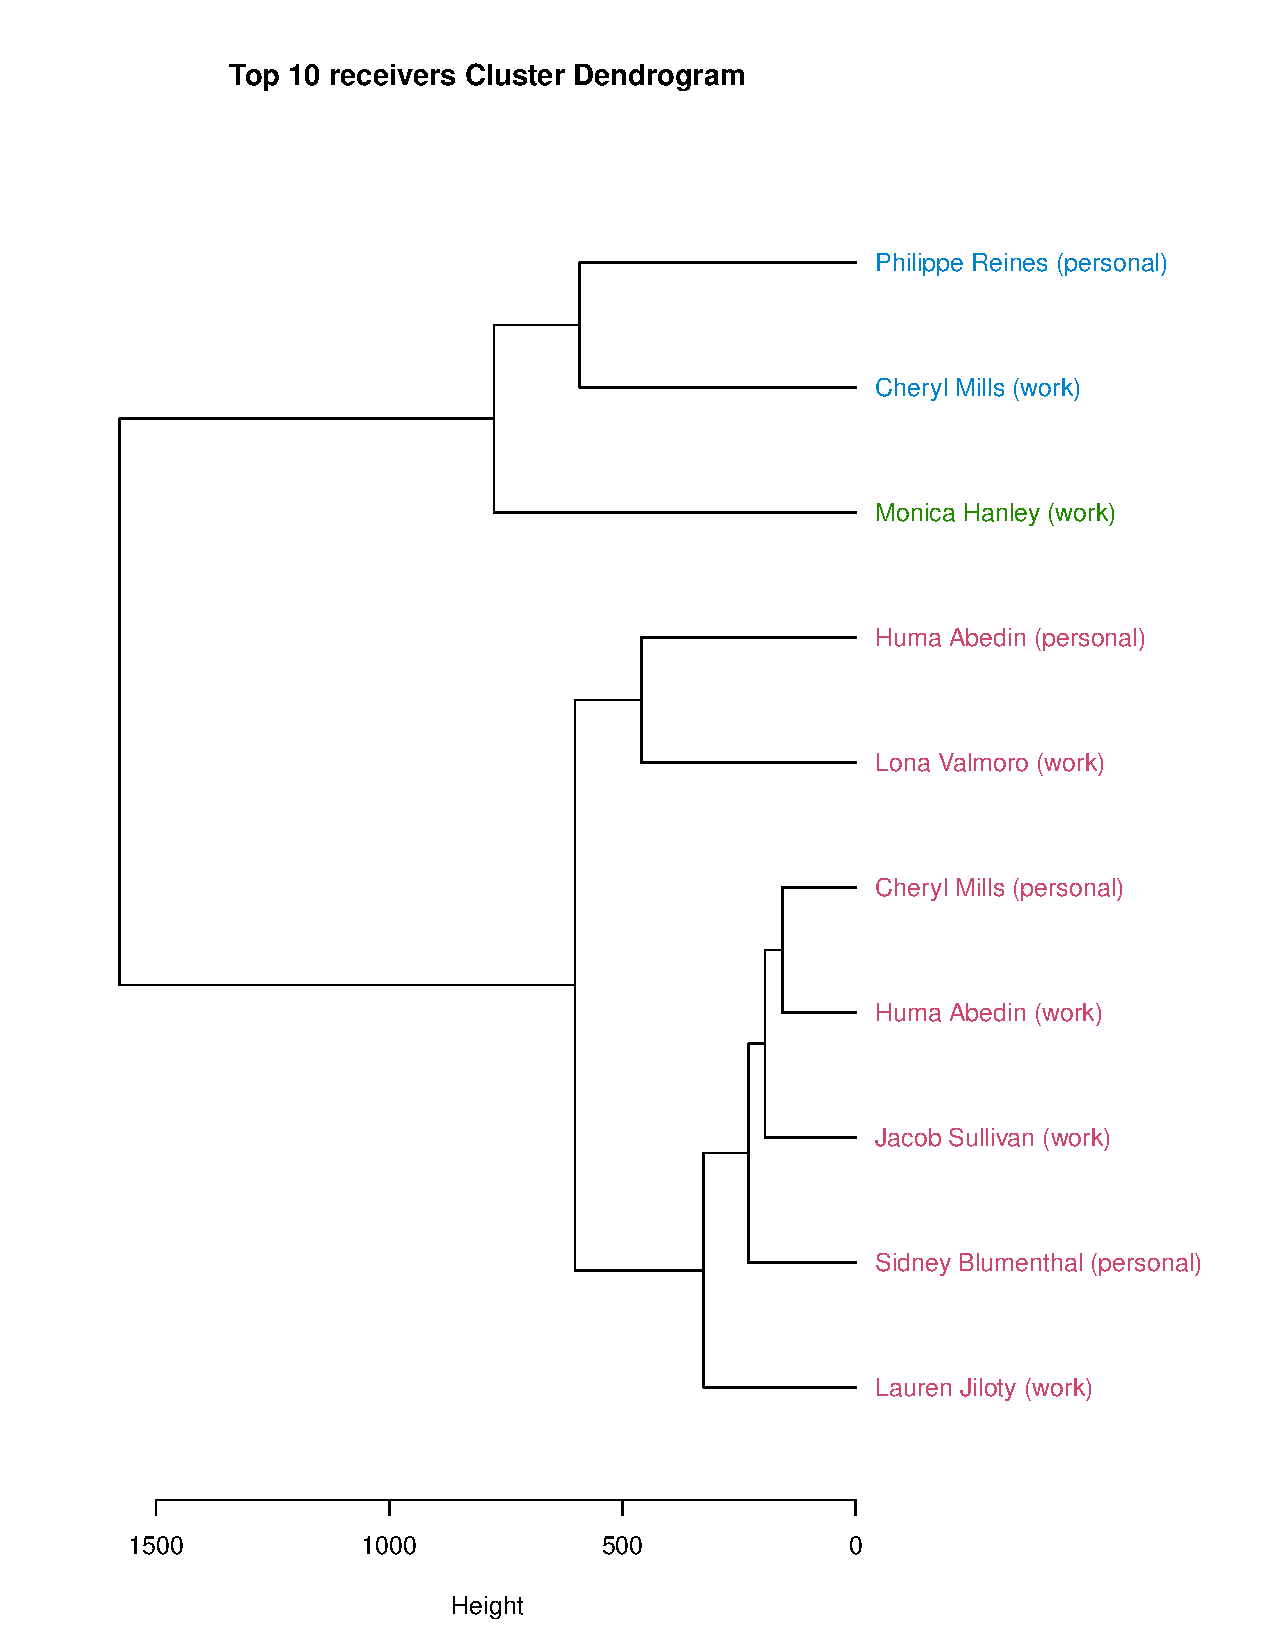
\includegraphics[width=10cm,height=10cm]
    {daitong_and_yihe/clusterp.pdf}
    \caption{Dendrogram of top 10 receiver accounts}
\end{figure}

We can also use K-means to determine the clusters. By plotting the within group sum of square versus K, we can see that K=2 or K=3 might be appropriate group numbers for this dataset.
\begin{figure}[h!]
    \centering
    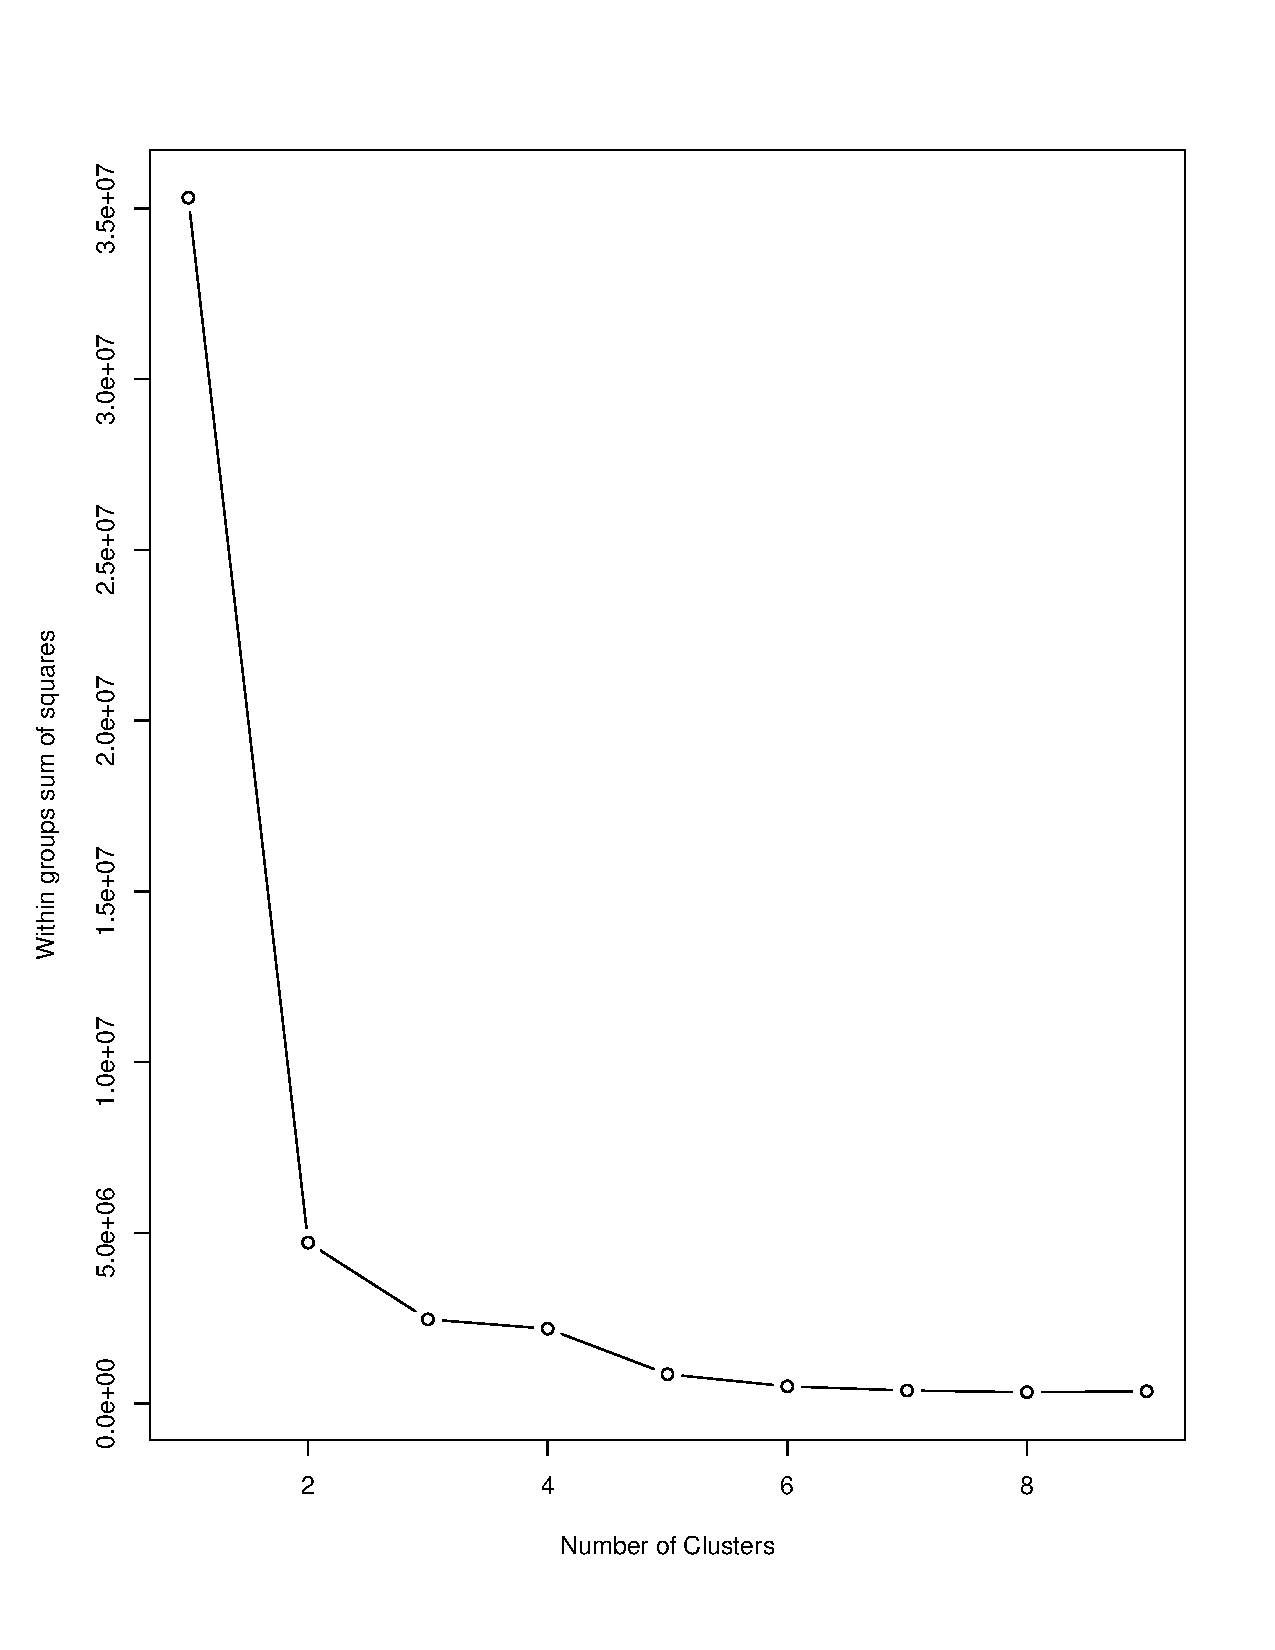
\includegraphics[width=10cm,height=10cm]
    {daitong_and_yihe/clusterd.pdf}
    \caption{Dendrogram of top 10 receiver accounts}
\end{figure}

The cluster plots with K=2 and K=3 can be shown in Figures 3 and 4 below. The x and y axes are represented by the first and second components from a PCA analysis. As we can see, the first two components explain more than 95\% of the variance, allowing the clusters to be well separated. 

The results of K-means agree with the results from hierarchical clustering. With K=2, we have Sidney Blumenthal (personal), Cheryl Mills (personal) and Monica Hanley (work) in one group (call it Cluster 1) and the other accounts in the second group. With K=3, we have Sidney Blumenthal (personal), Cheryl Mills (personal) in group one, Monica Hanley (work) in group two, and the other accounts in group 3.

\begin{figure}[h!]
    \centering
    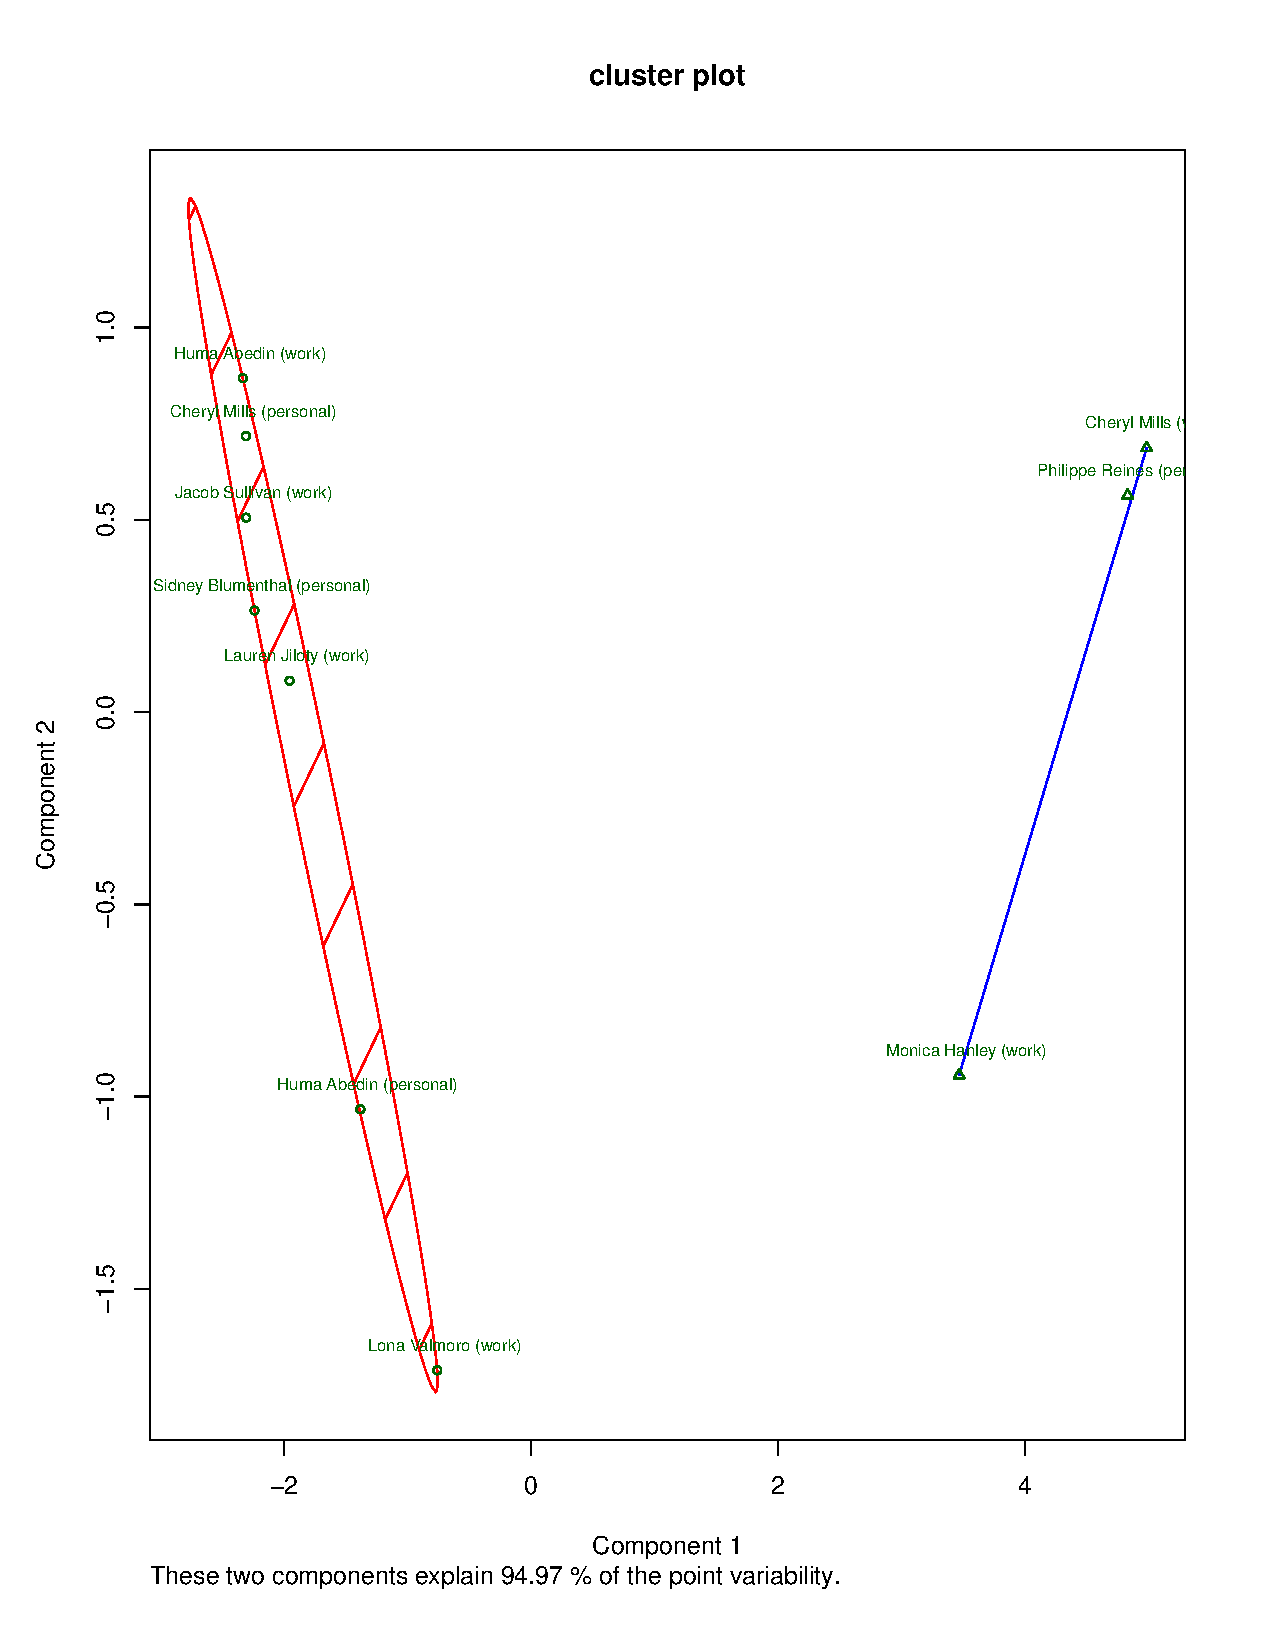
\includegraphics[width=10cm,height=9cm]
    {daitong_and_yihe/c2.pdf}
    \caption{Cluster Plot with K=2}
\end{figure}

\begin{figure}[h!]
    \centering
    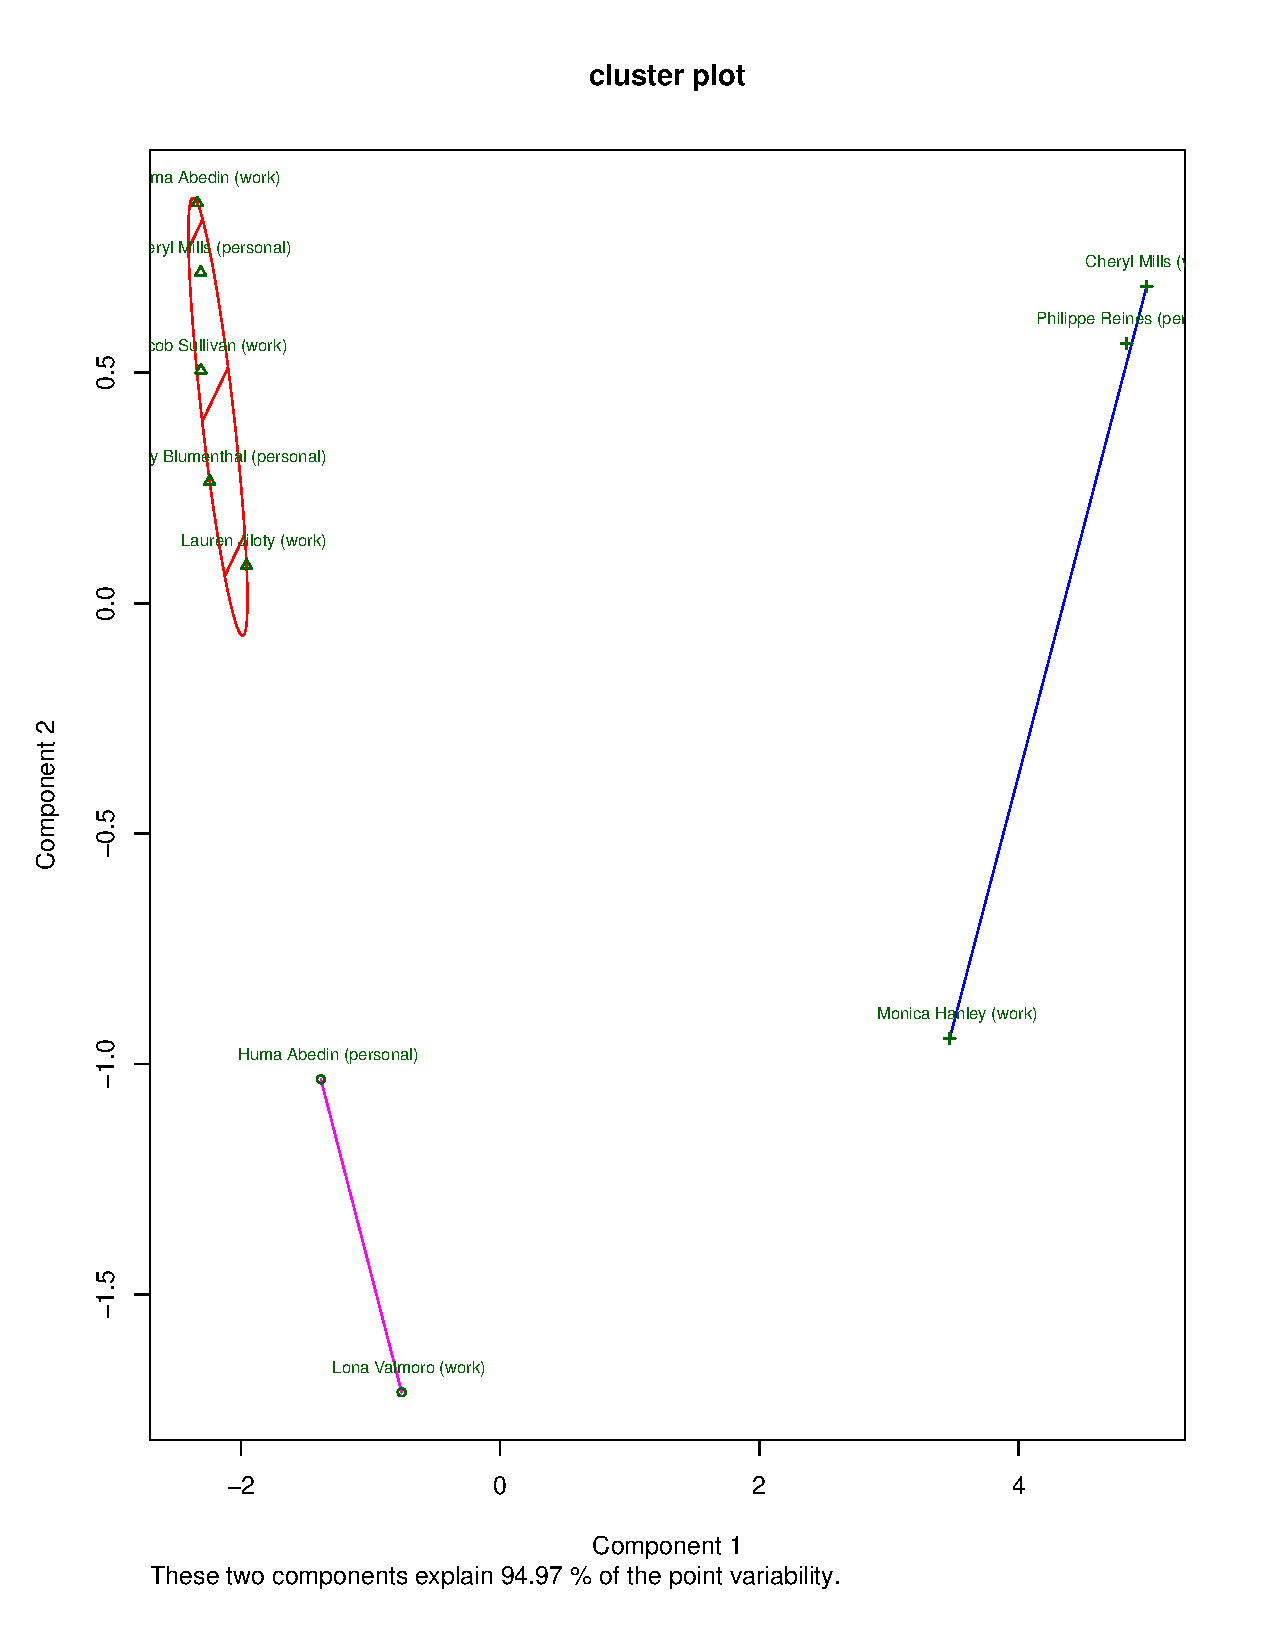
\includegraphics[width=10cm,height=9cm]
    {daitong_and_yihe/c3.pdf}
    \caption{Cluster Plot with K=3}
\end{figure}

\newpage
Furthermore, we can inspect the most frequent words mentioned by Clinton to each cluster of receivers. Below are the top 5 words related to each of the two clusters. Both clusters share common words like Benghazi, sensitive and house, although Hillary used the term 'agreement' more often with the journalist and the lawyer and the term 'release' more frequently with her aides and advisors. 

\begin{center}
\begin{tabular}{ |p{3cm}|p{3cm}|| p{3cm}|p{3cm}|  }
 \hline
 \multicolumn{4}{|c|}{Top 5 Most Frequent Words} \\
 \hline
 Words (Cluster 1)  & Percentage of Occurance & Words (Cluster 2) & Percentage of Occurance\\
 \hline
 benghazi & 0.76\% & release  & 0.701\% \\
 house &  0.68\% & benghazi & 0.56\% \\
 sensitive & 0.65\% & house & 0.53\%\\
 information & 0.63\% & information & 0.47\%\\
 agreement & 0.57\% &  sensitive  & 0.46\% \\
 \hline
\end{tabular}
\end{center}
=======
Using the emails datasets, there are 1906 number of people who have received emails from Hillary. We selected 10 receivers who have received highest numbers of emails from Clinton directly.
A simple word cloud for all 10 documents can be seen in Figure. \ref{fig:wcloud}
\begin{figure}[h!]
    \centering
    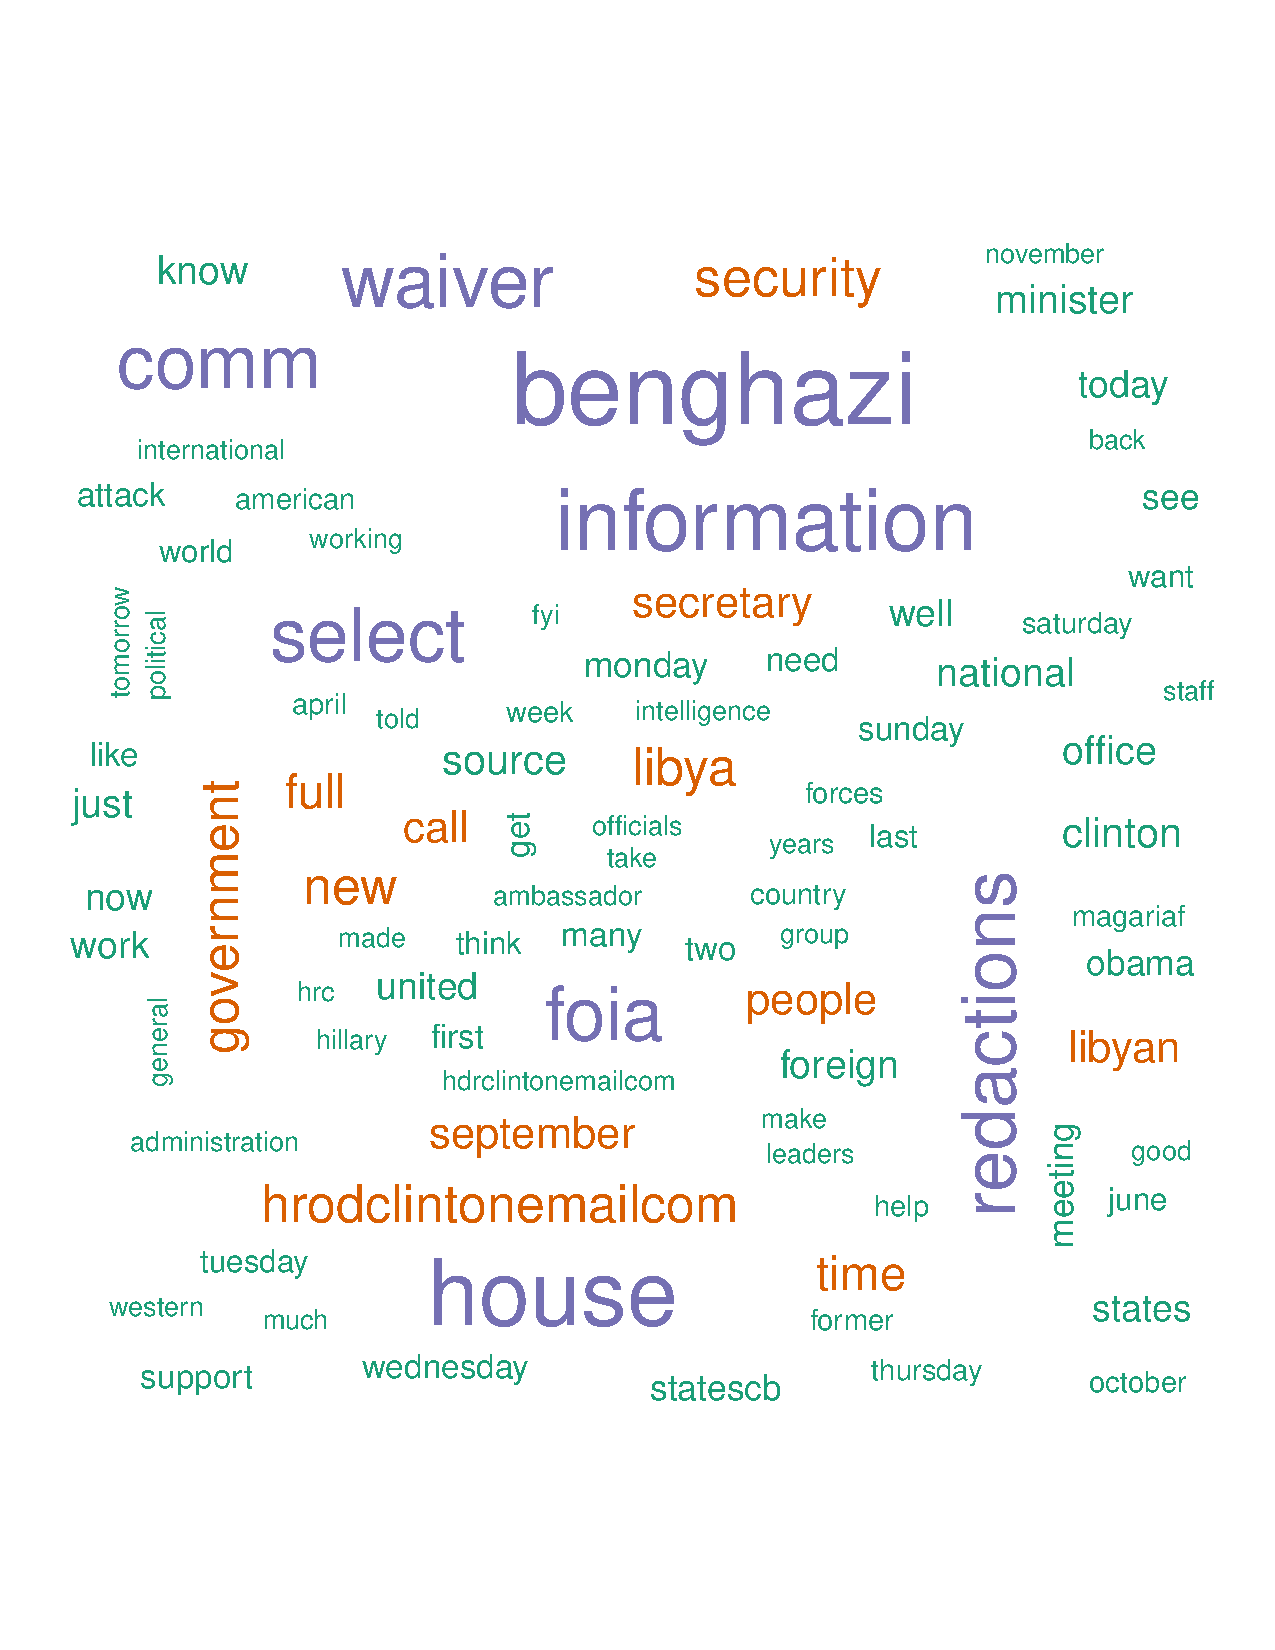
\includegraphics[width=10cm,height=10cm]
    {daitong_and_yihe/wcloud}
    \caption{Word Cloud of Emails}
    \label{fig:wcloud}
\end{figure}

\newpage
\subsection*{Clustering Results}
After obtaining the matrix containing the distances between each documents, we tried two methods: hierarchical clustering and K-means. 
\\
For hierarchical clustering, we have used ward.D method or the Ward's minimum variance method. Figure \ref{fig:dendr} is a cluster dendrogram of the top 10 email accounts. The different colours represents the grouping. The height represents the distance between each document. For example, at distance of 800 we can separate the group in pink and others. The calculation of distance is explained in the section above.
\begin{figure}[h!]
    \centering
    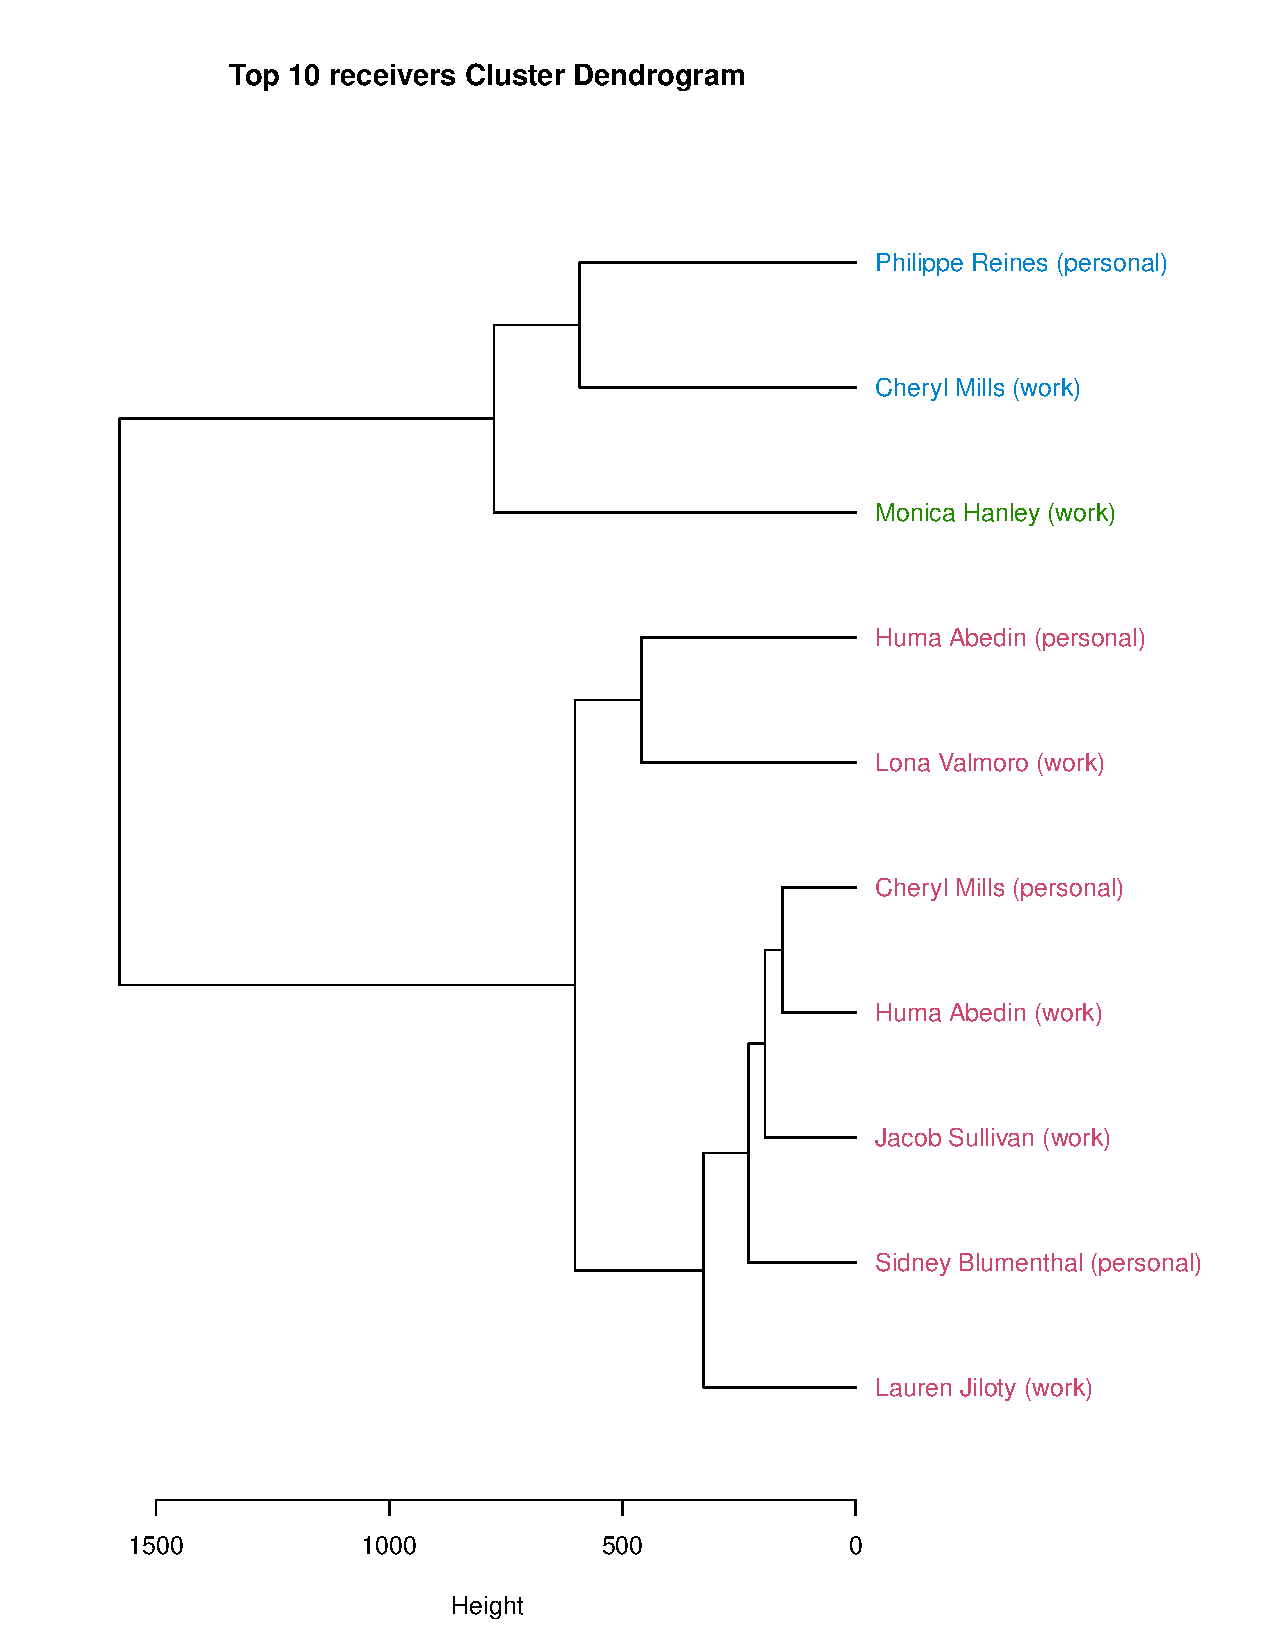
\includegraphics[width=10cm,height=10cm]
    {daitong_and_yihe/clusterp}
    \caption{Dendrogram of top 10 receiver accounts}
    \label{fig:dendr}
\end{figure}

We can also use K-means to determine the clusters. By plotting the within group sum of square errors versus K, we can see from Figure \ref{fig:determine} that K=2 or K=3 might be appropriete group numbers for this dataset.
\begin{figure}[h!]
    \centering
    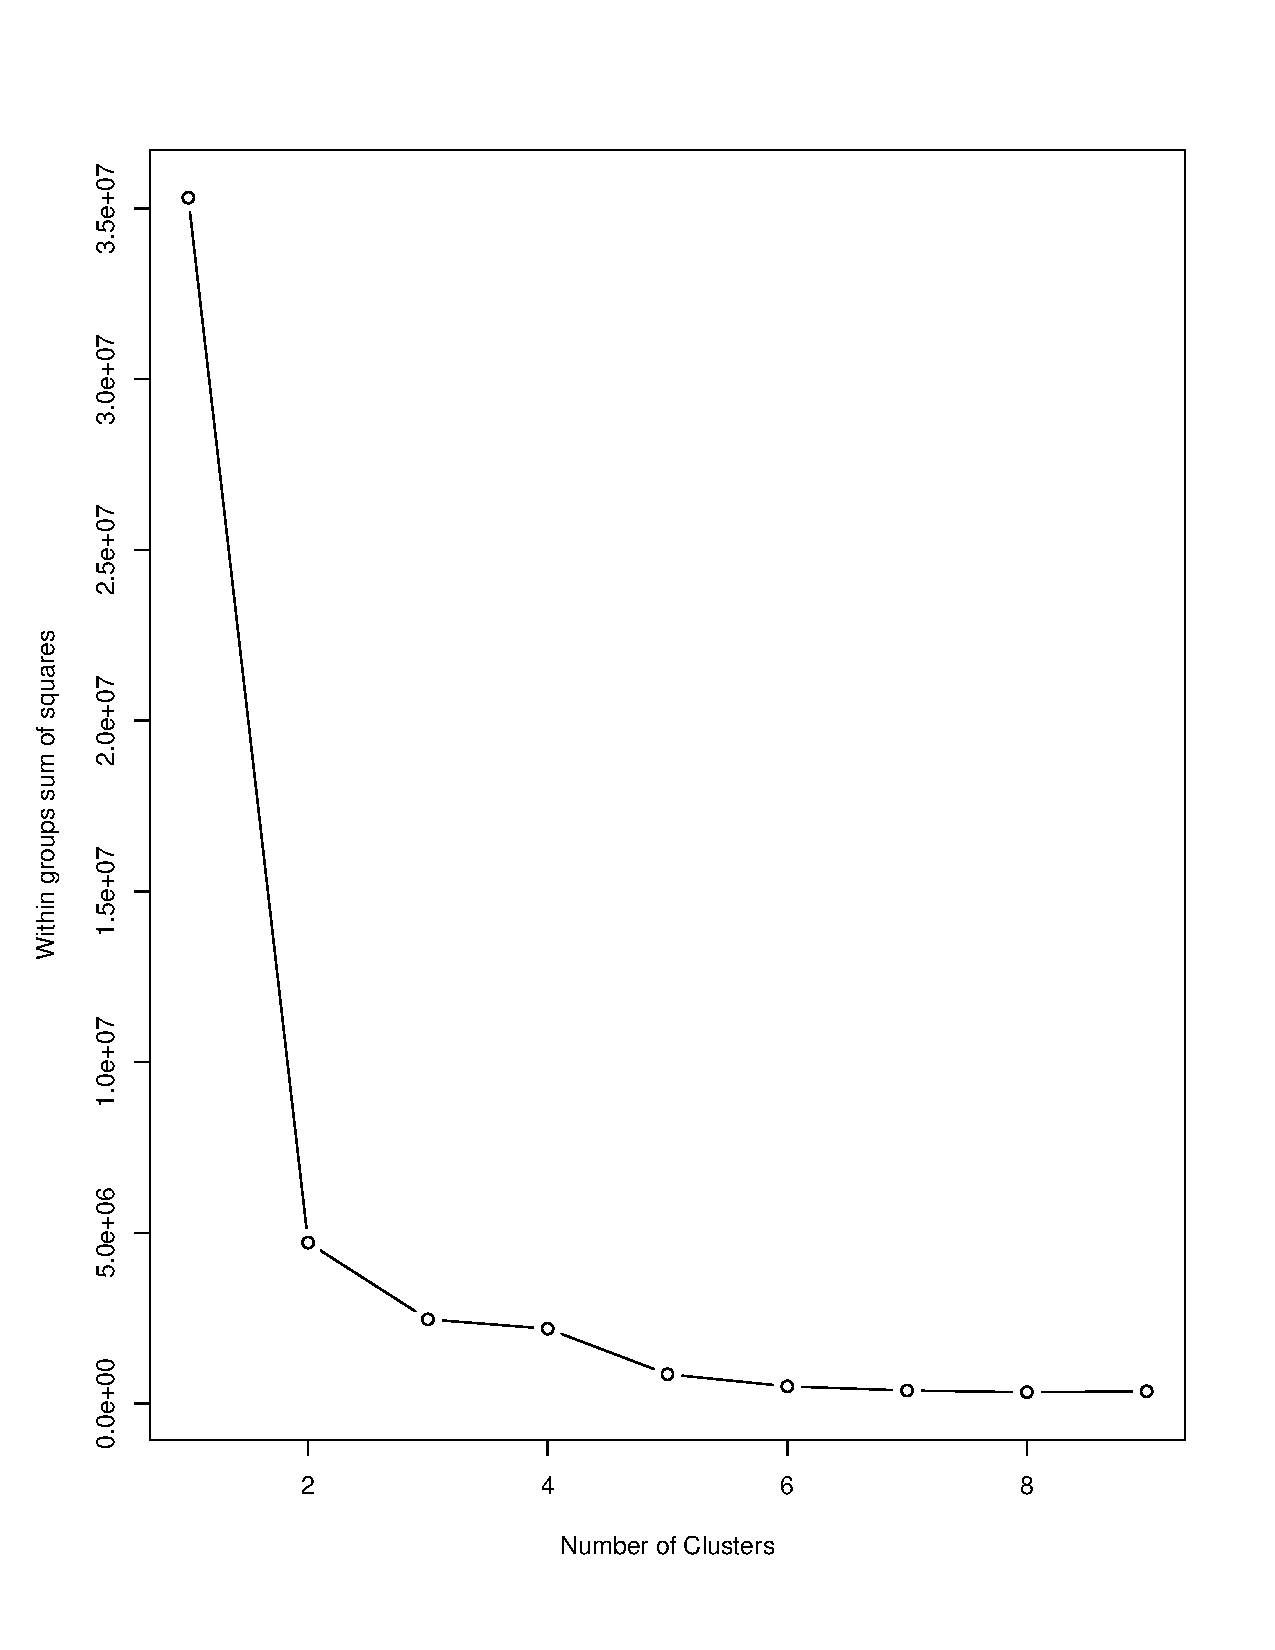
\includegraphics[width=10cm,height=10cm]
    {daitong_and_yihe/clusterd}
    \caption{Within group sum of square errors versus K=1,...,9}
    \label{fig:determine}
\end{figure}


The cluster plots with K=2 and K=3 can be shown in Figure 3 and 4 below. The x and y axis are represented by the first and second component from the PCA analysis. As we can see that the first two components explain more than 95\% of the variance, allowing the clusters to be well separated. 
\\
The results of K-means agree with the results from hierachical clustering. With K=2, we have Sidney Blumenthal (personal), Cheryl Mills (personal) and Monica Hanley (work) in one group (call it Cluster 1) and other accounts in the second group. With K=3, we have Sidney Blumenthal (personal), Cheryl Mills (personal) in group one, Monica Hanley (work) in group two and other accounts in group 3. The clusters can be seen in Figure.\ref{fig:c2} and \ref{fig:c3}.

\begin{figure}[h!]
    \centering
    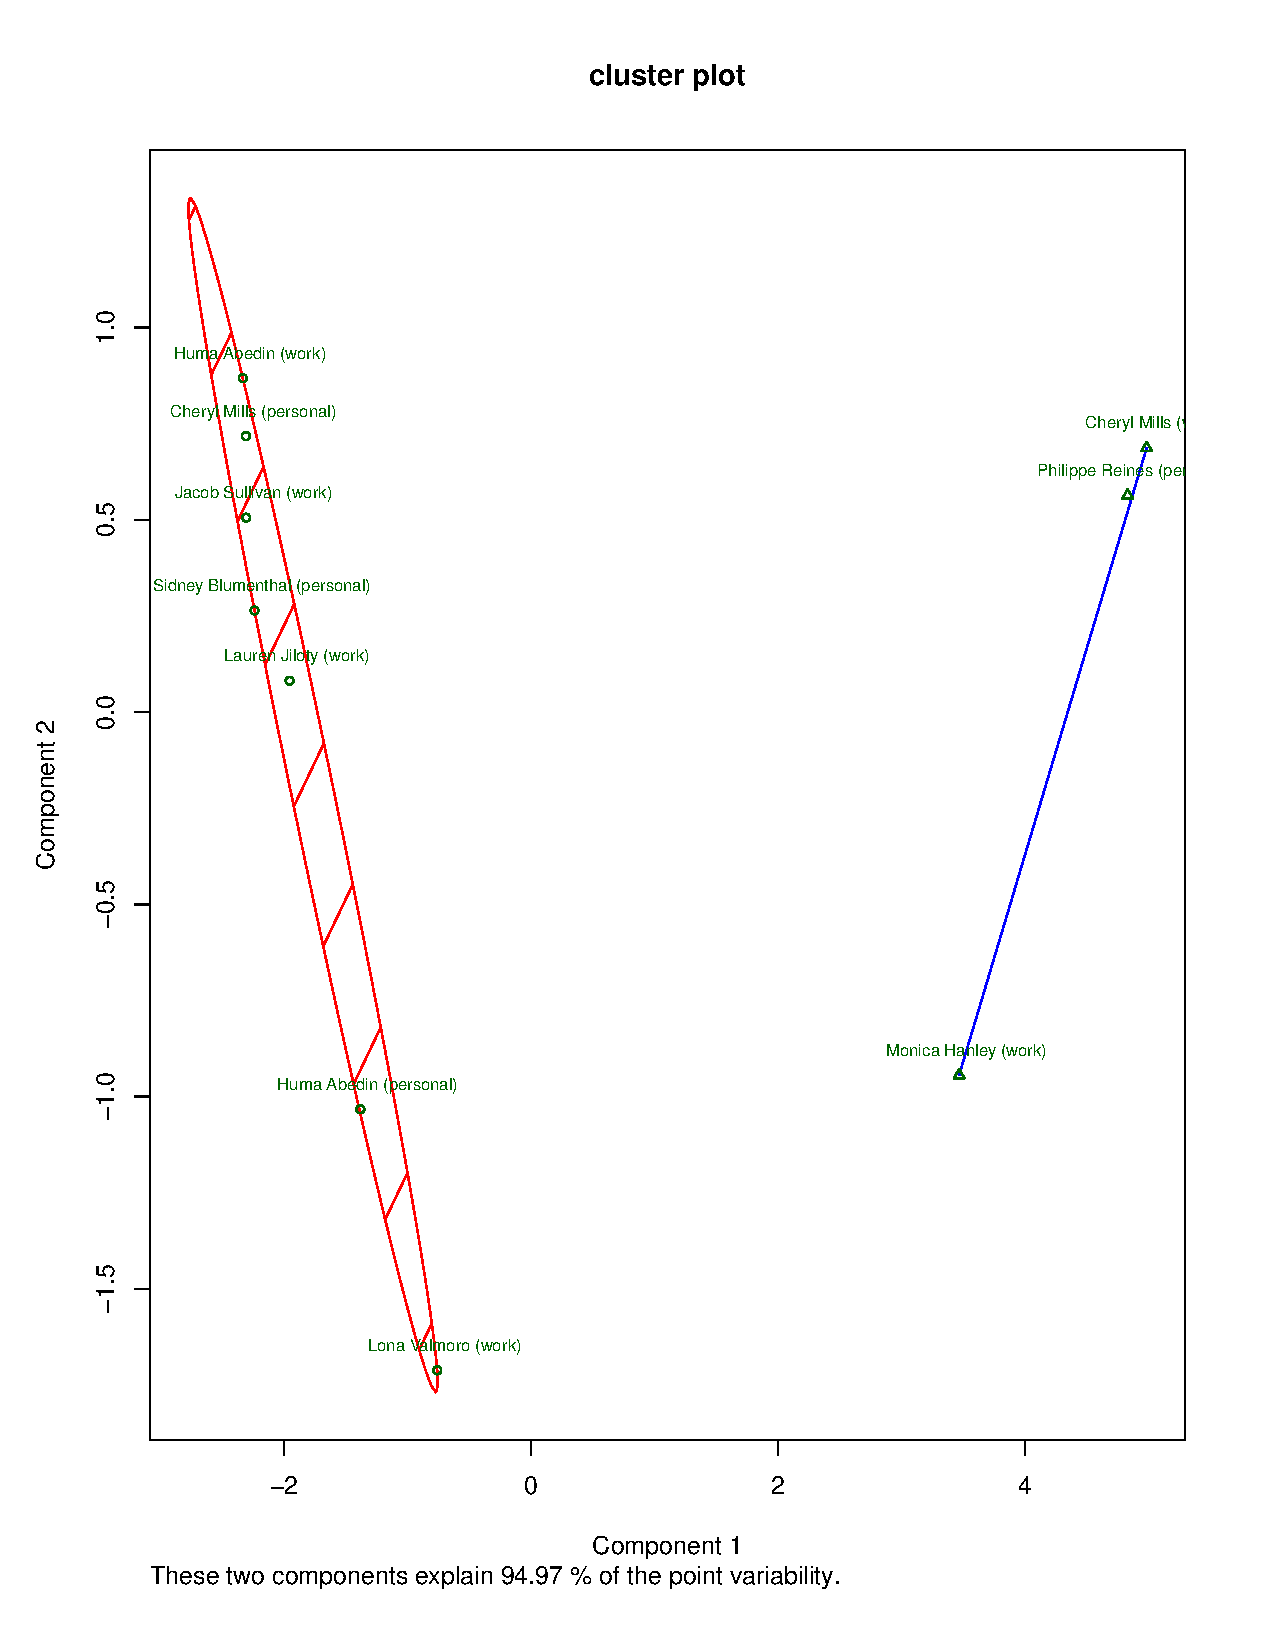
\includegraphics[width=10cm,height=9cm]
    {daitong_and_yihe/c2}
    \caption{Cluster Plot with K=2}
    \label{fig:c2}
\end{figure}

\begin{figure}[h!]
    \centering
    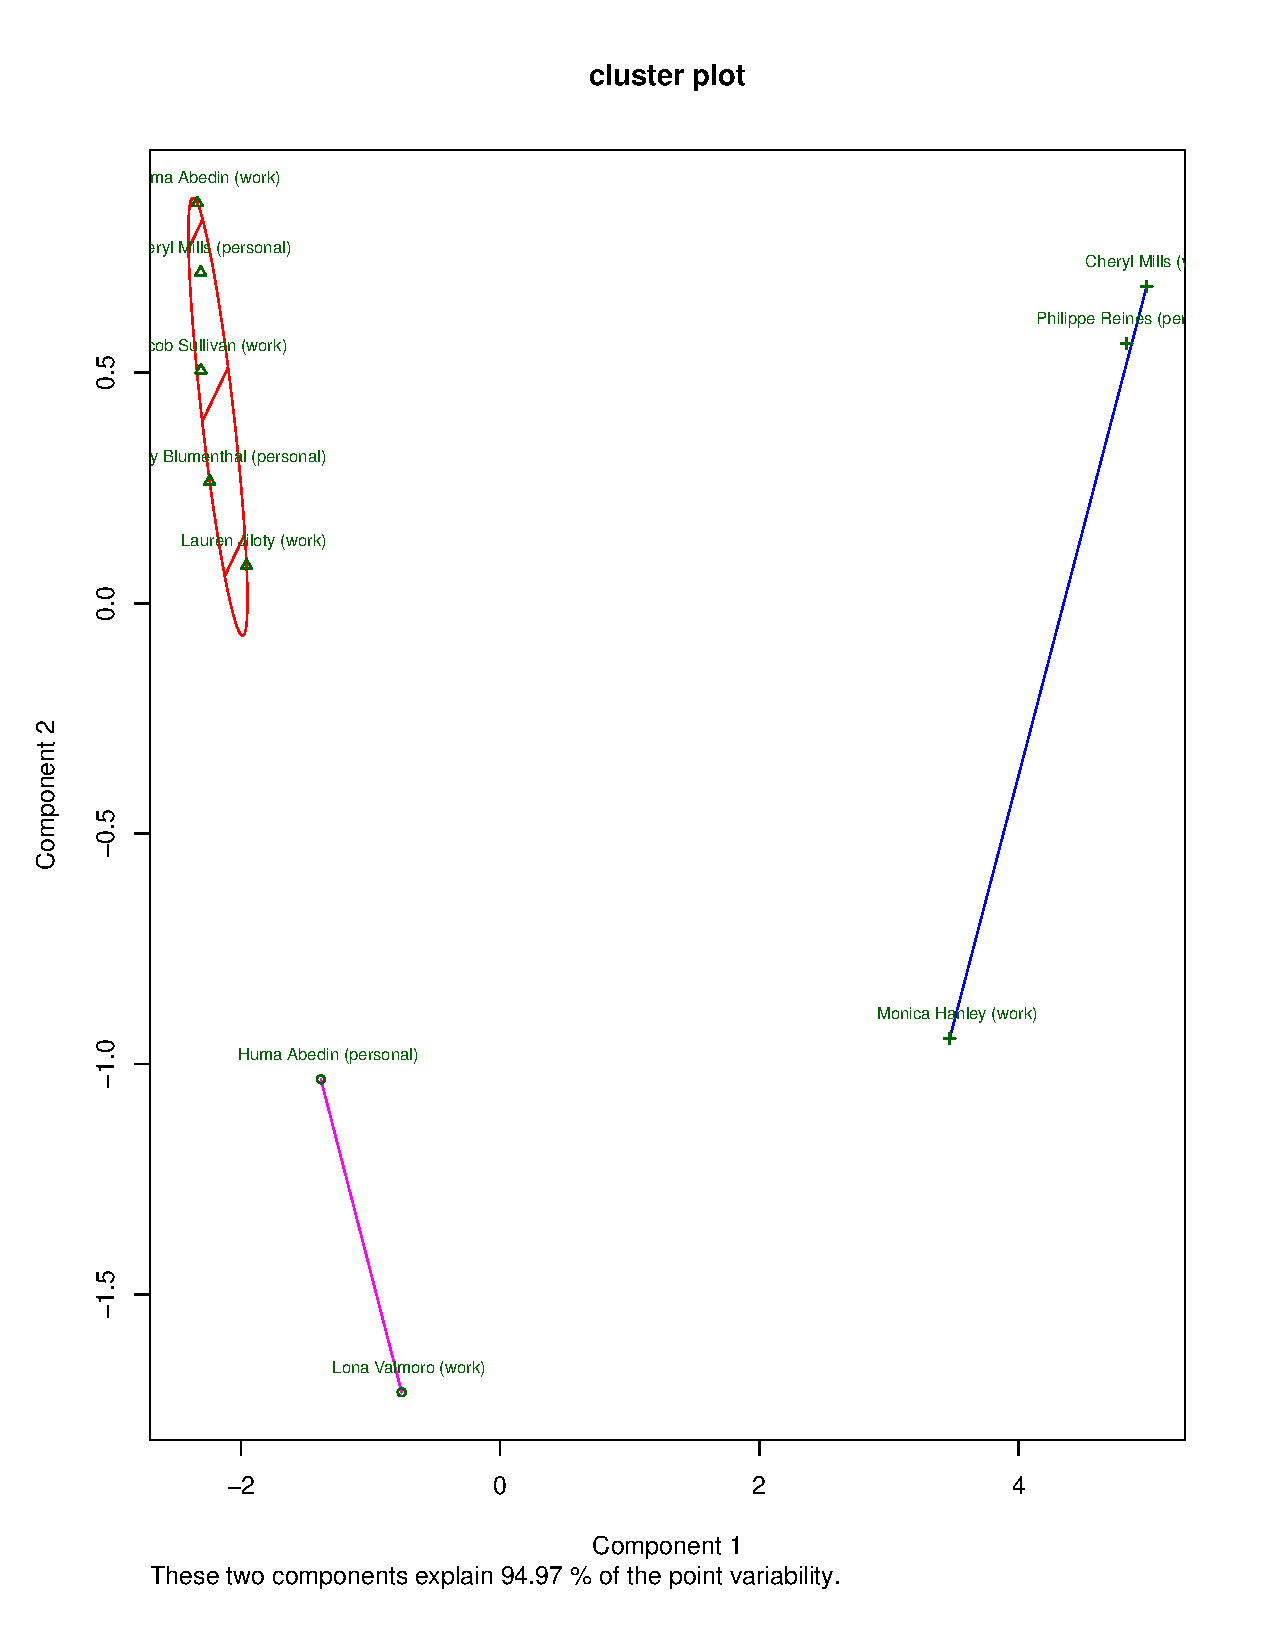
\includegraphics[width=10cm,height=9cm]
    {daitong_and_yihe/c3}
    \caption{Cluster Plot with K=3}
    \label{fig:c2}
\end{figure}

\newpage
Further more, we can inspect the most frequent words mentioned by Clinton to each cluster of receivers. Below is the top 5 words used by each of the two clusters. Both clusters share common words like Benghazi, sensitive and house; though Hillary talked about the term 'agreement' more with the journalist and the lawyer; and the term 'release' more with her aides and advisors. 
\\

\begin{center}
\begin{tabular}{ |p{3cm}|p{3cm}|| p{3cm}|p{3cm}|  }
 \hline
 \multicolumn{4}{|c|}{Top 5 Most Frequent Words} \\
 \hline
 Words (Cluster 1)  & Percentage of Occurance & Words (Cluster 2) & Percentage of Occurance\\
 \hline
 benghazi & 0.76\% & release  & 0.701\% \\
 house &  0.68\% & benghazi & 0.56\% \\
 sensitive & 0.65\% & house & 0.53\%\\
 information & 0.63\% & information & 0.47\%\\
 agreement & 0.57\% &  sensitive  & 0.46\% \\
 \hline
\end{tabular}
\end{center}
>>>>>>> 378d580337365fac7b06723b194db1f30dcc9538
